\section*{\textbf{II. Experimental Design}}
\addcontentsline{toc}{section}{II.\hspace{0.15in} Experimental Design}

\begin{wrapfigure}{R}{2in}
    \includegraphics[width=2in]{multilayer.png}
    \caption{An illustration of the photonic crystal used in our sensor}
    \label{fig:multilayer}
\end{wrapfigure}
\hspace{0.15in}
The process of design for this experiment relies heavily on the use of a 15 milimeter right prism and our photonic crystal. The photonic crystal is composed of 3 bilayers of TiO2 and SiO2. The dielectric function of TiO2 is taken as $\epsilon_{TiO2} = 4.84 + 0.0007i$ and the dielectric function of SiO2 is taken as $\epsilon_{SiO2} = 2.1316 + 0.0001i$. It should be noted that the imaginary parts of each dielectric function may not be accurate due to the values being not well known and have been included to introduce some form of loss that fits the results of prior experiments. Figure 3 illustrates the structure of the multilayer.


The sensor is composed of three different parts: the primary stage, two beams, and the flowcell stage.  One of the two beams holds our laser and a focusing lens while the other holds the CCD and captures the reflected beam. Normally the laser light is too intense to pick up the surface mode in the reflected image. We attach a neutral density filter (d=3.5, see Figure \ref{fig:beams}) to the CCD to reduce the intensity and this allows us to image the surface mode. 

% Picture of beams, central stage, and flowcell stage
\begin{figure}[h]
    \begin{center}
    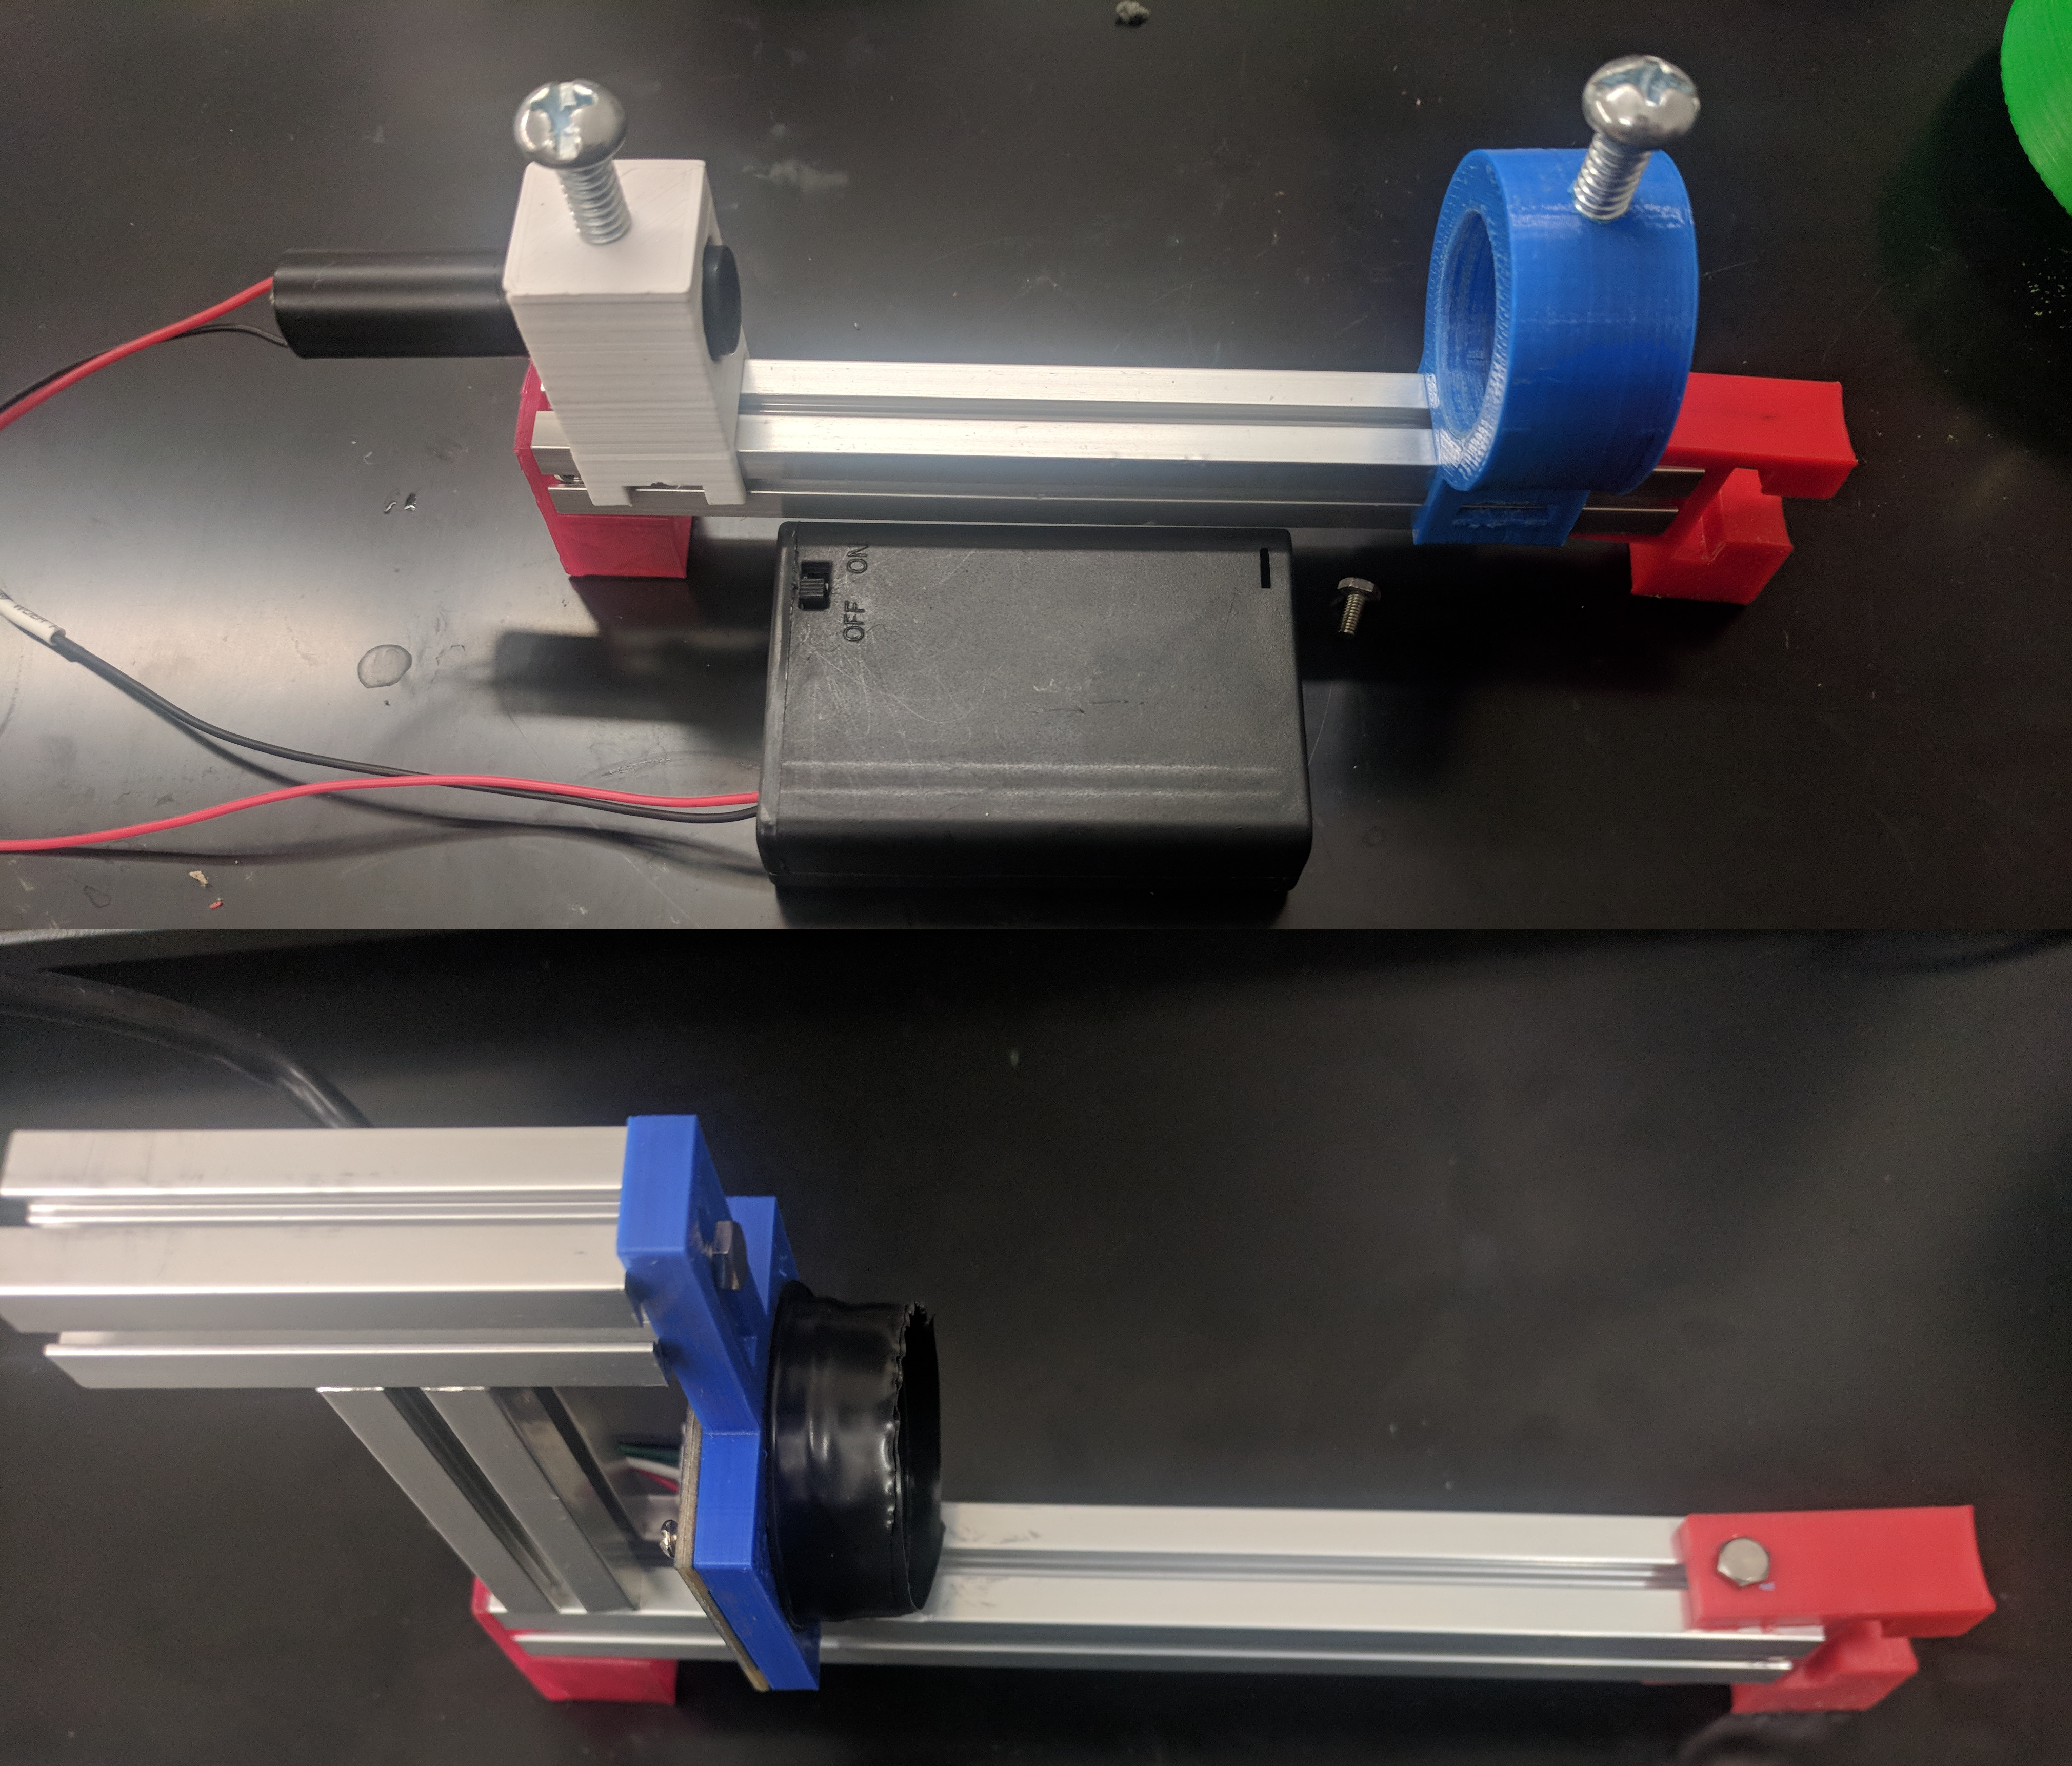
\includegraphics[width=0.6\textwidth]{arms.png}
    \caption{Top: the beam holding the laser and focusing lens. Bottom: the beam holding the camera and neutral density filter.}
    \label{fig:beams}
    \end{center}
\end{figure}

Each beam is a 15cm x 10mm x 10mm aluminum MakerBeam. Attached on the left side of each beam in Figure \ref{fig:beams} is a foot used to keep the beams level with the central platform. On the right side of each beam is a 3D printed connector used to attach the beams to the primary stage. The beams are capable of rotating around the axis that keeps these connectors in place, allowing a larger range of coupling angles for the laser-multilayer system.


The primary stage (see the green 3D printed fixture in Figure \ref{fig:centralstage}) acts as the center about which the incident beam can be coupled to the prism and then reflected onto the CCD. The design of this stage allows different types of multilayers to be used since the incident laser can be oriented at nearly any angle. The flowcell stage (see the blue 3D printed piece bolted into the primary stage in Figure \ref{fig:centralstage}) is a modular piece that is attached to the primary stage with four bolts. The prism, multilayer, and flowcell chamber are all strapped together on this stage via two pairs of 3D printed braces and hex screws. The modular nature of this piece of the sensor is valuable since multiple designs can be used to achieve the generate BSWs and it only takes between 40 minutes to an hour to print off each flowcell stage.

\begin{figure}[h]
\begin{center}
    \includegraphics[width=0.7\textwidth]{central_stage.png}
    \caption{Primary stage and flowcell stage of our sensor. The green round 3D printed fixture underneath the flowcell is the primary stage which the two beams are attached to via a small divot in the back. The blue 3D printed piece mounted to the primary stage is the flowcell stage. The glass prism, multilayer, and flowcell chamber are attached atop the flowcell stage with the use of hex screws and 3D printed braces.}
    \label{fig:centralstage}
\end{center}
\end{figure}


To flow liquids through the chamber the whole fixture must be water tight. To accomplish this we designed the flowcell so that a rubber gasket could be fit around the chamber. When the braces are tightened there is no liquid loss at the interface during operation, however the chamber is made of PLA and liquid will leak through the plastic after a few hours. The two apertures on top of the flowcell are used for inflow and outflow. To ensure no leaks occur when flushing the chamber we wrapped each aperture with electrical tape before attaching our tubing. 

\begin{figure}[h]
\begin{center}
    \includegraphics[width=0.7\textwidth]{flowcell.jpg}
    \caption{The flowcell stage, prism, multilayer and flowcell chamber. A rubber gasket is set in a groove around the chamber so that when the braces are tightened the interface between the multilayer and flowcell is liquid tight.}
    \label{fig:flowcellstage}
\end{center}
\end{figure}

The decision to print a flowcell stage separate from the primary stage allows the design to be tinkered with without wasting too much time. Using our 3D printers the primary stage takes about nine hours to print, while the flowcell stage only takes about fourty minutes to one hour. This is useful because the position of the glass prism (used to couple incident light to the multilayer) can be more conveniently oriented to produce BSWs. A diagram illustrating the coupling angle required for our multilayer is illustrated in Figure \ref{fig:couplingangle}. From that diagram it is easy to see how awkward an angle is needed for the sensor to operate, but the ability to translate the prism's bed by printing off another flowcell stage makes it natural to orient the laser at the coupling angle. The next section details how the coupling angle is computed and how data is collected by imaging the surface mode.

\begin{figure}[t!]
\begin{center}
    \includegraphics[width=\textwidth]{couplingangle.png}
    \caption{The geometry behind our coupling angle when the flowcell chamber is filled with water. The lines normal to the left leg and hypotenuse of the triangle represent the surface normals of the prism. The line $40^\circ$ from the left leg surface normal and $66^\circ$ from the hypotenusal surface normal represent the path of the incident light. The laser needs to be oriented about $5^\circ$ off of parallel with the hypotenusal face of our prism. It is quite an awkward angle, but a different flowcell stage can be printed to make reaching this coupling angle more natural by translating the prism's bed upward.}
    \label{fig:couplingangle}
\end{center}
\end{figure}